%!TEX root = ../../Master.tex
\subsection{Hardware} % (fold)
\label{sub:hardware}

Systemet består af tre hardware komponenter - en robot, et kamera og en laptop.
En oversigt over systemet er illustreret i \autoref{fig:hardware}.
I dette afsnit vil hver af disse hardware komponenter blive beskrevet.

\fixme{Ændre 'Figure' til 'Figur'}

\begin{figure}[h]
\centering
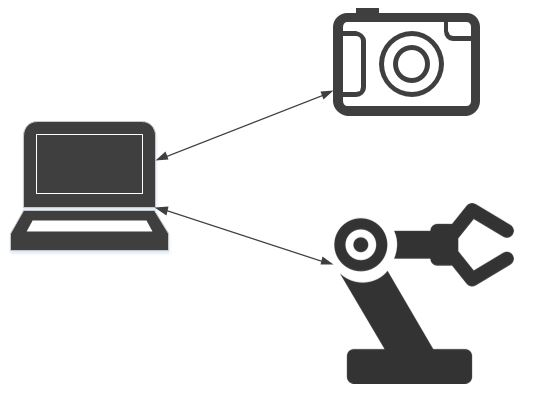
\includegraphics[scale=0.5]{images/hardware}
\caption{Systemoversigt med hardware komponenter}
\label{fig:hardware}
\end{figure}

\subsubsection{Robot} % (fold)
\label{subsub:robot}

\fixme{Ændre 'section' til 'afsnit'}

Systemet anvender en robotarm til at flytte klodserne fra bordets midte til den side, hvor klodsen er blevet sorteret til.
Robotten, som anvendes i systemet, er den i \autoref{sub:crust_crawler} allerede beskrevne AX-12A Smart Robotic Arm fra CrustCrawler Robotics.
Robotten styres fra systemets laptop ved at tildele de enkelte joints (rotationsled) en vinkel, som de så indstiller sig til.

% subsubsection robot (end)

\subsubsection{Kamera} % (fold)
\label{subsub:camera}

Systemet anvender et kamera til detektion af klodserne samt vurdering af disses farver.
Kameraet, som anvendes i systemet, er et D-Link DCS 930L.
Kameraet har en opløsning på $640 \times 480$ pixels og tilsluttes via ethernet.
Kameraet er tilsluttet systemets laptop, som henter billeder fra kameraet, når det er nødvendigt.

% subsubsection camera (end)

\subsubsection{Laptop} % (fold)
\label{subsub:laptop}

Systemet anvender en laptop til styring af robotten samt det nødvendige billedbehandling.
Denne laptop kører med ubuntu som operativsystem, og har ROS kørende.
Systemets laptop er i besidelse af mindst en USB port og ethernet port.

% subsubsection laptop (end)

% subsection hardware (end)